%%%%%%%%%%%%%%%%%%%%%%%%%%%%%%%%%%%% Chapter Template

\chapter{2D steady simulations} 	% Main chapter title
\label{Chapter1} 		% For referencing the chapter elsewhere, usage \ref{Chapter1}

%%%%%%%%%%%%%%%%%%%%%%%%%%%%%%%%%%%%

The initial goal was to identify the factors that contribute to the VMG's superior efficiency compared to the R1V4 and make the necessary adjustments.

The first step involved identifying the parameters that respond to various flight conditions. Following that, a low-fidelity approach using XFLR5 was employed to compute the 2D aerodynamic coefficients, providing insights into the disparities between the airfoils. Subsequently, Fluent CFD software was utilized to obtain a more precise assessment of the aerodynamic coefficients for each airfoil during actual flight conditions.

This is a reference to an article \cite{example}.

%%%%%%%%%%%%%%%%%%%%%%%%%%%%%%%%%%%%%%%%%%%%%%%%%%%%%%%%%%%%%%%%%%%%%%%%%%%%%%%%
%%%%%%%%%%%%%%%%%%%%%%%%%%%%%%%%%%%% SECTION 1 %%%%%%%%%%%%%%%%%%%%%%%%%%%%%%%%%
%%%%%%%%%%%%%%%%%%%%%%%%%%%%%%%%%%%%%%%%%%%%%%%%%%%%%%%%%%%%%%%%%%%%%%%%%%%%%%%%

\section{Kite flight modelling}
\label{sec:Ch1.1}

Example
\begin{figure}[H]
    \centering
    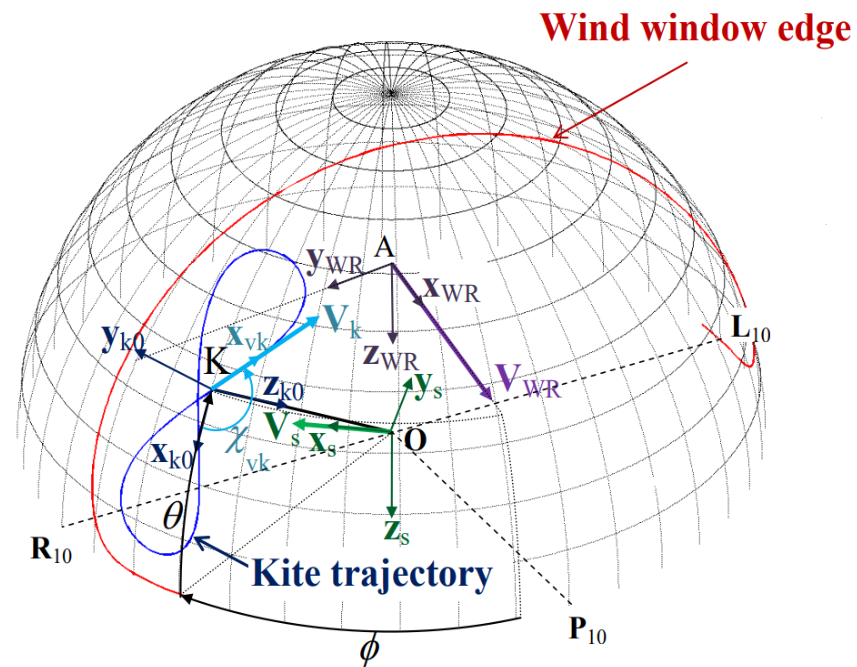
\includegraphics[width=0.7\textwidth]{figures/2D steady simulations/kite flight modeling 1.png}
    \caption{Speeds \& angles decomposition}
    \label{fig:Kite_flight_modelling}
\end{figure}


\begin{wrapfigure}{r}{0.6\textwidth}
\centering
    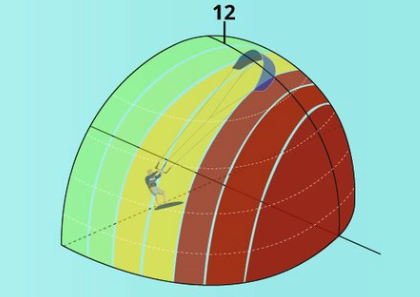
\includegraphics[width=0.5\textwidth]{figures/2D steady simulations/kite flight modeling 3.png}
    \caption{The wind window}
    \label{fig:The_wind_window}
\end{wrapfigure}

%%%%%%%%%%%%%%%%%%%%%%%%%%%%%%%%%%%%%%%%%%%%%%%%%%%%%%%%%%%%%%%%%%%%%%%%%%%%%%%%
%%%%%%%%%%%%%%%%%%%%%%%%%%%%%%%%%%%% SECTION 2 %%%%%%%%%%%%%%%%%%%%%%%%%%%%%%%%%
%%%%%%%%%%%%%%%%%%%%%%%%%%%%%%%%%%%%%%%%%%%%%%%%%%%%%%%%%%%%%%%%%%%%%%%%%%%%%%%%
\section{The different phases}
\label{sec:Ch1.3}

Example

%%%%%%%%%%%%%%%%%%%%%%%%%%%%%%%%%%%% SUBSECTION 1

\subsection{The upwind}
\label{sub:Ch1.3.1}

example
%%%%%%%%%%%%%%%%%%%%%%%%%%%%%%%%%%%% SUBSECTION 2

\subsection{The downwind}
\label{sub:Ch1.3.1}

Example

%%%%%%%%%%%%%%%%%%%%%%%%%%%%%%%%%%%%%%%%%%%%%%%%%%%%%%%%%%%%%%%%%%%%%%%%%%%%%%%%
%%%%%%%%%%%%%%%%%%%%%%%%%%%%%%%%%%%% SECTION 3 %%%%%%%%%%%%%%%%%%%%%%%%%%%%%%%%%
%%%%%%%%%%%%%%%%%%%%%%%%%%%%%%%%%%%%%%%%%%%%%%%%%%%%%%%%%%%%%%%%%%%%%%%%%%%%%%%%

\section{Experimental data }
\label{sec:Ch1.2}

\begin{table}[H]
    \center
    \begin{tabular}{|l|l|l|l|}
        \hline
            & $\alpha_{s, WT} ($°$) $ & $V_{WT} (knots) $ & $V_{S} (knots) $ \tabularnewline
        \hline
        Upwind & 39,5 & 14,0 & 22,5  \tabularnewline
        \hline
        Downwind & 155,0 & 14,0 & 31,5  \tabularnewline
        \hline
    \end{tabular}
    \caption{Average data from Axel's race}
    \label{tab:Average_data_from_Axels_race}
\end{table}